\chapter{Introduction}
\label{chapter 1}
\ifpdf
    \graphicspath{{Chapter1/Figs/}{Chapter1/Figs/PDF/}{Chapter1/Figs/}}
\else
    \graphicspath{{Chapter1/Figs/Vector/}{Chapter1/Figs/}}
\fi
In the last three centuries humankind experienced three different industrial revolutions that deeply modified every aspect of society, not only changing production and economic models, but also generating new cultural movements and wide political unrests across the world. \\
The First Industrial Revolution began at the end of the 18th century in Great Britain. The design of efficient steam engines and the use of coke as fuel allowed to highly increase production, especially in iron making and textile industries, and to reduce transportation cost and time. \\
After a slowdown in important innovations in the middle of 19th century, in the last decades of the century many new inventions (e.g. electrical power, petroleum refining, rubber vulcanization) produced a continuous improvement in manufacturing industry. This period is known as the Second Industrial Revolution and culminated with Henry Ford’s product standardization and mass production, inspired by Taylor’s “The Principles of Scientific Management”. Ford’s model (known as Fordism) brought to a massive production and consumption increase, generating both huge wealth and widespread social tensions. \\ 
At the end of the 1940s, AT\&T Bell Laboratories invented the transistor. This was the first step to the design and production of microprocessors, which are the basis of the Third Industrial Revolution. In particular, in the last decades of 20th century, computers led to process automation and system control and monitoring, generating a growth of productivity, efficiency and quality in manufacturing. Processor capability development and diffusion in every field of the human activities have gone along with data storage capacity increase, which in turn led to the problem of information extraction from huge, complex, and scattered databases. \\
Manufacturing has been deeply influenced by the recent advancements in digital technologies. Innovative production and process control techniques started to spread in the last decade; the most remarkable ones are cyber-physical systems, Internet of Things, digital twin, big data analytics, and cloud computing \cite{ZhongRayandXuXunandKlotzEberhardandNewmanStephen}. The challenge of implementing the digitalization in manufacturing led to define a new high-tech strategy by the German government in 2011, soon taken as example by the rest of the world. In the same year, the term “Industrie 4.0” (i.e. Industry 4.0) was introduced \cite{WollschlaegerMartin2017TFoI}, implying that these technological developments are considered so significant that it is now widely acknowledged we are entering in the Fourth Industrial Revolution. 
\section{Industry 4.0 components}
\label{Industry 4.0 components}
\begin{center}
\textit{What does the Fourth Industrial Revolution consist of?}
\end{center}
To understand the complex landscape of Industry 4.0, I will summarize the definitions of the main facets of this new manufacturing model, then I will outline how these concepts are linked to each other.
\paragraph{Cyber-Physical System (CPS)}
A CPS is defined in \cite{LeeJay2015ACSa} as “\textit{transformative technologies for managing interconnected systems between its physical assets and computational capabilities}”. In other words, CPS refers to a system where physical objects and software elements are linked to interact and exchange information. 
In \cite{LeeJay2015ACSa}, two main functional components of a CPS are identified, which are (a) an advanced connectivity able to manage data acquisition and transfer in real-time, and (b) a cyber-space where information is extracted and consequent decisions are taken. Then in the same paper a 5-level (“5C”) architecture is proposed as guideline for implementation of CPS in a manufacturing application. 
\paragraph{Internet of Things (IoT)}
The term IoT refers to a production or service model where various sensorized objects (i.e. “Things”) are connected, creating a network through which they collect and share data in real-time. The implementation of an IoT system introduces many challenges. A reliable and affordable automatic identification technology is required to made the objects “smart”; RFID technology is a viable answer, and it’s already actively used for identifying various objects in warehouses, production shop floors, logistics companies, distribution centers, retailers, and disposal/recycle stages. Also, a secure, high speed, and high bandwidth wireless communication standard has to be adopted to manage the huge amount of data generated by the sensors embedded with the objects; 5G technology is a possible, yet controversial, candidate to address this problem.
\paragraph{Digital Twin (DT)}
The DT is “\textit{the virtual and computerized counterpart of a physical system that can be used to simulate it} (i.e. the physical system) \textit{for various purposes, exploiting a real-time synchronization of the sensed data coming from the field}” \cite{NegriElisa2017ARot}. The deep difference with a simple simulation model is that a DT is not a static but a dynamic representation (at a desired level of detail) of the system: it imitates and changes in accordance with the real system. However, this relationship is not one-directional, having the DT that, in turn, while running in parallel, influences the real system, allowing to foresee the process evolution through simulation and to design improvements. 
\paragraph{Big Data Analytics (BDA)}
Big Data, as written in the HACE theorem \cite{XindongWu2014Dmwb}, “\textit{starts with large-volume, heterogeneous, autonomous sources with distributed and decentralized control, and seeks to explore complex and evolving relationships among data}”. The data characteristics stated by the definition are typical of any data output in CPS, where different sensors, spread across the production lines, gather and send data to a central system. The amount of collected data requires the use of modern analysis techniques to extract meaningful information, such as Data Mining and Process Mining. 
\paragraph{Cloud Computing (CC)}
Cloud computing is a general term that indicates the offer by Internet-related companies (like Google, Microsoft, or Amazon) of computational and storage services through scalable resources over the web. The scalability of resources allows organizations to reduce initial investments and to adjust the business digital capabilities as needs arise. The most significant concerns about cloud computing, apart from technological challenges such as load balancing, scalability and availability, and compatibility among different clouds, are related to privacy issues and security. 
\paragraph{ }
\begin{figure}[h] 
\centering    
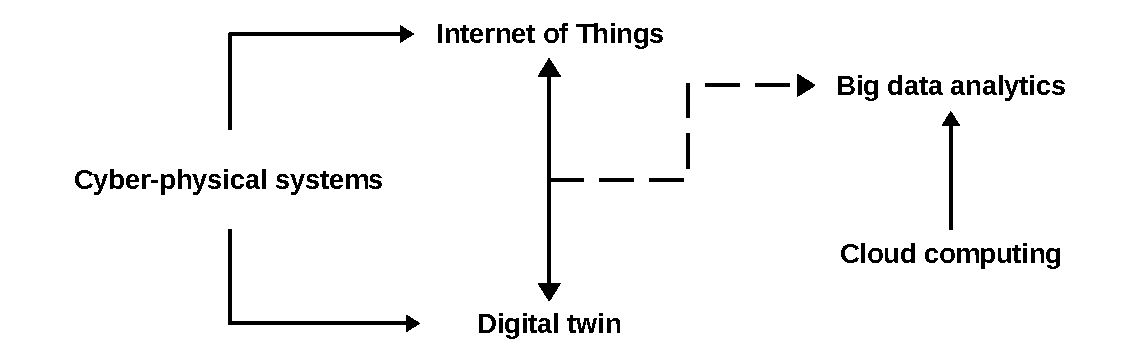
\includegraphics[width=1\textwidth]{Industria 4 schema}
\caption{Industry 4.0 scheme}
\label{fig:Industria 4 schema}
\end{figure}
Although these concepts do not have well-defined borders, and even partially overlap, figure \ref{fig:Industria 4 schema} was included to suggest a logical connection among them. The main aspect that jumps out from the previous definitions is that IoT and DT are two sides of the same coin, which is CPS: IoT can be considered the hardware side and DT the software side of a CPS. The CPS monitoring and the coordination of its parts are performed using BDA techniques, which are hosted on digital environments capable of storing and analyzing huge amount of data (i.e. CC).\\
Ultimately, information extraction and exchange are the glue that brings all the Industry 4.0 facets together. Indeed, the main innovative side that characterize the Fourth Industrial Revolution is the exploitation of huge amount of data, aiming to automatically improve efficiency and quality in manufacturing contexts. 
\section{Tools of Big Data Analytics}
BDA works as a bridge between the hardware side and the software side of a CPS, extracting information from the data collected by sensors embedded in the real system (IoT) and from data obtained by simulations run on the digital copy (DT). In general, the activity of obtaining information from big data volumes is called Knowledge Discovery in Databases (KDD), defined in \cite{ChoudharyAlokK.2009Dmim} as “\textit{the nontrivial process of identifying valid, novel, potentially useful, and ultimately understandable patterns in data}”. KDD does not belong to a specific field of application, indeed it is a framework that can also adopted in manufacturing contexts. 
\begin{figure}[h] 
\centering    
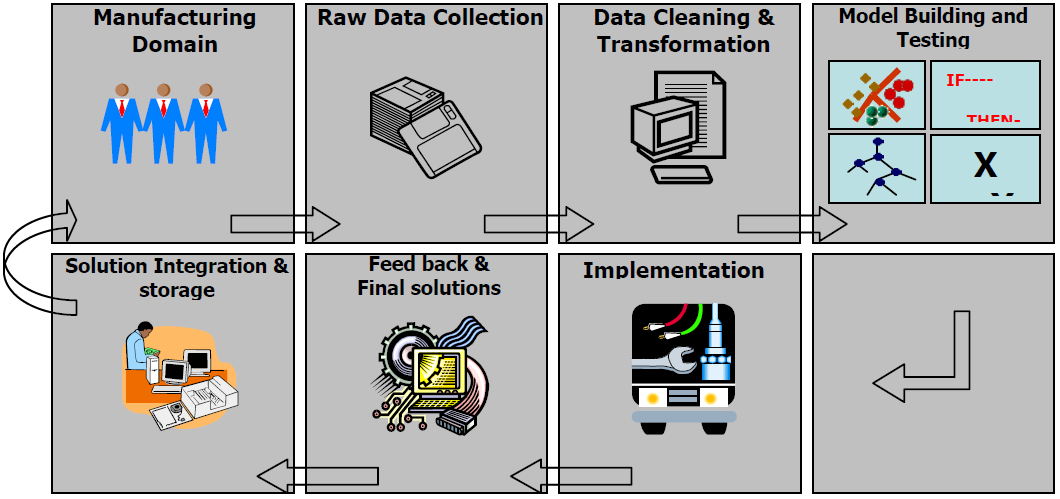
\includegraphics[width=1\textwidth]{KDD}
\caption{KDD in manufacturing \cite{ChoudharyAlokK.2009Dmim}}
\label{fig:KDD in manufacturing}
\end{figure} 
As figure \ref{fig:KDD in manufacturing} shows, KDD includes many steps: 
\begin{enumerate}
\item Understanding the manufacturing domain: preliminary research of the manufacturing sector which the data come from, and specification of the analysis goals
\item Collection of the data: raw data gathering from different sources
\item Data cleaning, pre-processing and transformation: data pre-processing to remove noise, replace missing values and redundancies, and selection of a dataset structure appropriate for data mining algorithms application 
\item Data integration: integration of data from heterogeneous sources
\item Selection of Data Mining area (see \ref{Data Mining}): selection of the Data Mining technique to use for the data analysis
\item Selection of the appropriate data mining algorithm: selection of the Data Mining algorithms to use for the data analysis
\item Interpretation and Visualization: study of the results and preparation of graphs to support the conclusions
\item Implementation of discovered knowledge: execution of the required system modifications and feedback collection 
\item Knowledge storage, reuse and integration into manufacturing system: storage of the acquired know-how in sight of future reuse
\end{enumerate}
\subsection{Data Mining}
\label{Data Mining}
The core of KDD is Data Mining (DM), that is the usage of specific algorithms for identifying patterns in data to uncover hidden relationships (Descriptive DM) and foresee outcomes (Predictive DM). It is possible to distinguish some DM main macro-areas:
\begin{itemize}
\item \textbf{Characterization \& Discrimination}: this DM branch aims to summarize data to provide a concise and information-rich description of the analyzed system. \\It is widely used in manufacturing contexts to address quality control problems or to get a overall sight of a process.
\item \textbf{Classification}: this DM branch aims to map (i.e. classify) the data into one of many different predefined classes. \\In manufacturing contexts, it is particularly used to classify defects and to perform online control chart pattern recognition.
\item \textbf{Clustering}: this DM area branch aims to map the data into one of many different not-predefined classes; these classes are called clusters, characterized by being natural grouping of data items based on similarity metrics. \\Some examples of manufacturing usage are its application to study supply chain and order picking routines, and to design part families and machine cells in cellular manufacturing.
\item \textbf{Prediction}: this DM area branch aims to build and use models to foresee the class of unlabelled samples, or to assess the value or value range of an attribute that a given sample is likely to have. \\It is widely used in manufacturing contexts, for example to design efficient resource maintenance policies, predicting the deterioration of components and machines.
\item \textbf{Association}: this DM branch aims aims to identify relationships patterns among items in a database, not based on inherent properties of the data, but rather on frequency of data-items co-occurrences. \\An example of its application in a manufacturing context is the usage of association to identify an efficient disposition of items stocked in a warehouse.
\end{itemize}
These DM macro-areas are deeply interwined and different approaches can be concurrently applied to explore data and extract meaningful information. \\
\subsection{Process Mining}
In recent years, data analysis research brought to the design of highly specialized and efficient DM algorithms, devised for specific areas of application. This leaning towards specialization lead to the definition of different DM fields, whose developments are separately pursued, even if mutual influences are still present. Some DM field examples are Text Mining, that aims to extract information from written sources, and Image Mining, that focuses on studying hidden patterns in pictures and photos. Among the others, in the late 1990s, Process Mining has been introduced.\\
Process Mining (PM) develops across multiple disciplines beyond DM, involving also Artificial Intelligence research and business process modeling. PM has the purpose of "\textit{discover, monitor and improve real processes by extracting knowledge from event logs readily available in today's (information) systems}" \cite{VanDerAalstWil2012Pmm}, where event logs are data structures that register the events occurred during a process execution (see section \ref{Event logs}). \\As the definition suggests, there are three main types of PM \cite{Aalst16}:
\begin{figure}[h]
  \centering
  \begin{subfigure}[t]{0.9\textwidth}
    
\includegraphics[width=\textwidth]{process_discovery}
    \caption{ }
    \label{fig:process_discovery}   
  \end{subfigure}
  \begin{subfigure}[h]{0.9\textwidth}
    
\includegraphics[width=\textwidth]{conformance_checking}
    \caption{ }
    \label{fig:conformance_checking}   
  \end{subfigure}
  \begin{subfigure}[b]{0.9\textwidth}
    
\includegraphics[width=\textwidth]{model_enhancement}
    \caption{ }
    \label{fig:model_enhancement}   
  \end{subfigure}
  \caption{The three main Process Mining branches, highlighting input and output of each one}
\end{figure}
\begin{itemize}
\item \textbf{Process Discovery}\\As figure \ref{fig:process_discovery} shows, this PM branch focuses on extracting information from the event log in order to understand the logical dependencies among the activities constituting the process. In other words, it aims to build a process model (i.e. a model describing the system behavior) looking at what activities are performed on cases (i.e. jobs) passing through the system.
\item \textbf{Conformance Checking}\\As figure \ref{fig:conformance_checking} shows, this PM branch focuses on the comparison of the behavior of cases registered in an event log with the process behavior prescribed in an already existing process model, looking for mismatches between the actual system (i.e. the one recorded by the event log) and theoretical system (the one represented in the model).
\item \textbf{Model Enhancement}\\As figure \ref{fig:model_enhancement} shows, this PM branch focuses on the enrichment of an already existing process model through the analysis of an event log related to the same system. In particular, the process is studied from different points-of-view, such as the resource perspective (e.g. Organizational Mining, which gives insights about the social network structure of a system) and the case perspective (e.g. time an sequence analysis, that allows to easily build Gantt Charts). 
\end{itemize}
PM has been extensively applied in business and healthcare issues \cite{RojasEric2016Pmih}, and recent researches also tried to apply it to the manufacturing context. Indeed, event logs, which are the initial data source for any PM algorithm, are obtainable as outputs of sensors embedded in production lines, making PM a promising candidate as useful tool for CPS implementation (PM can be adapted to help in the DT construction) and maintenance. In particular, concerning the second part, it is critical to design efficient methods to keep DTs aligned with the real systems, and this thesis aims to suggest a new approach and to take the first steps into a new model updating process, employing the PM framework as a starting point. 
\section{Thesis structure}
In the second chapter the thesis scope is defined, exploring the state of the art and stating the dissertation goals. The third chapter describes the study boundaries, specifying what type of manufacturing systems, sensors, and process variations are taken into account. The fourth chapter focuses on the indicators used to monitor the process, explaining how they are extracted from event logs. The fifth and sixth chapters concern the experimental tests, respectively describing the simulated system characteristics and analyzing the indicator behaviors in the simulations. The seventh chapter summarizes the results shown in the previous chapter. 